\ifx\wholebook\relax\else
\input{../Common.tex}
\input{../macroes.tex}
\begin{document}
\fi

\chapter{Inspecting}\label{ch:turtleTeaching}


\subsection*{Inspecting  a Message's Result}

In fact, when you use the menu item \menu{Print It}, the message \ct{printString} is sent to the returned object. In \sq, every objects  know how to print itself, sometimes in a generic manner by just stating: aSomething, sometimes with much more elaborate description.

What is important to understand is that the highlighted text on the pane is not the returned object itself but a textual description of this object. There are several possibility to get the object itself. First we can just send directly a message. For example in the message  \ct{caro color darker} we send the message \ct{darker} to the result of the message \ct{caro color}. Second we can give a name to  the result of the message as shown in \tscrref{scr:naming} where the resulting color is named \ct{caroColor} and to which the message \ct{darker} is sent to. Finally we can 

\begin{scriptwithtitle}{Giving a name to a message result}\label{scr:naming}
| caro caroColor|
caro := Turtle new.
caroColor := caro color.
caroColor darker.
\end{scriptwithtitle}

\begin{figure}
\centerline{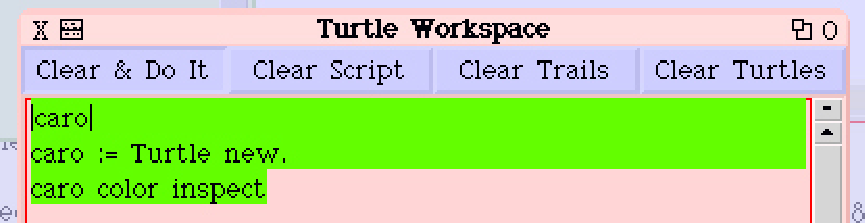
\includegraphics[width=8cm]{inspect}} 
\caption{\label{fig:inspect}}
\end{figure}


\begin{figure}
\centerline{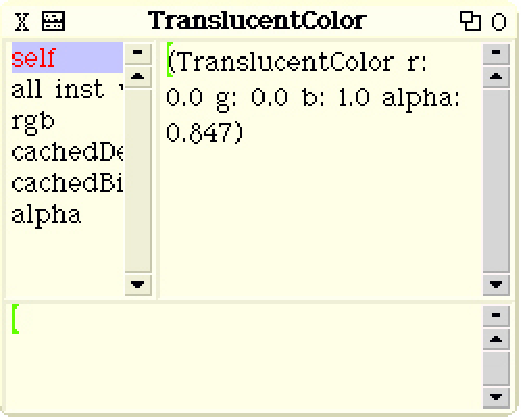
\includegraphics[width=6cm]{inspectedColor}} 
\caption{\label{fig:inspectedColor}}
\end{figure}




\ifx\wholebook\relax\else\end{document}\fi
